\chapter{Sicurezza delle reti wireless}
In questo capitolo verrà data inizialmente una breve panoramica sulle tecnologie wireless, seguita da una descrizione dettagliata del protocollo 802.11 (Wi-Fi) e delle sue insicurezze.

Introduciamo brevemente le due topologie di reti wireless (Figura \ref{img:wireless-topology}):
\begin{enumerate}
	\item \textbf{Modello infrastructure (o centralizzato)}. Questo tipo di rete ha origine da reti wireless commerciali, quindi vi è una stazione base detta \textit{Access Point} (AP), connessa in modo privato alla rete internet, alla quale si connettono tutti i dispositivi.
	\item \textbf{Modello ad-hoc (o distribuito)}. Questo tipo di rete si basa sulle comunicazioni multi-hop tra gli host della rete. Nel caso di rete locale il routing è diretto dal livello 7 perché è sufficiente l'indirizzo IP; nel caso di rete multi-hop, invece, il routing è quello classico, quindi vi sono tutti i problemi relativi agli attacchi.
\end{enumerate}
\begin{figure}[htbp]
	\centering
	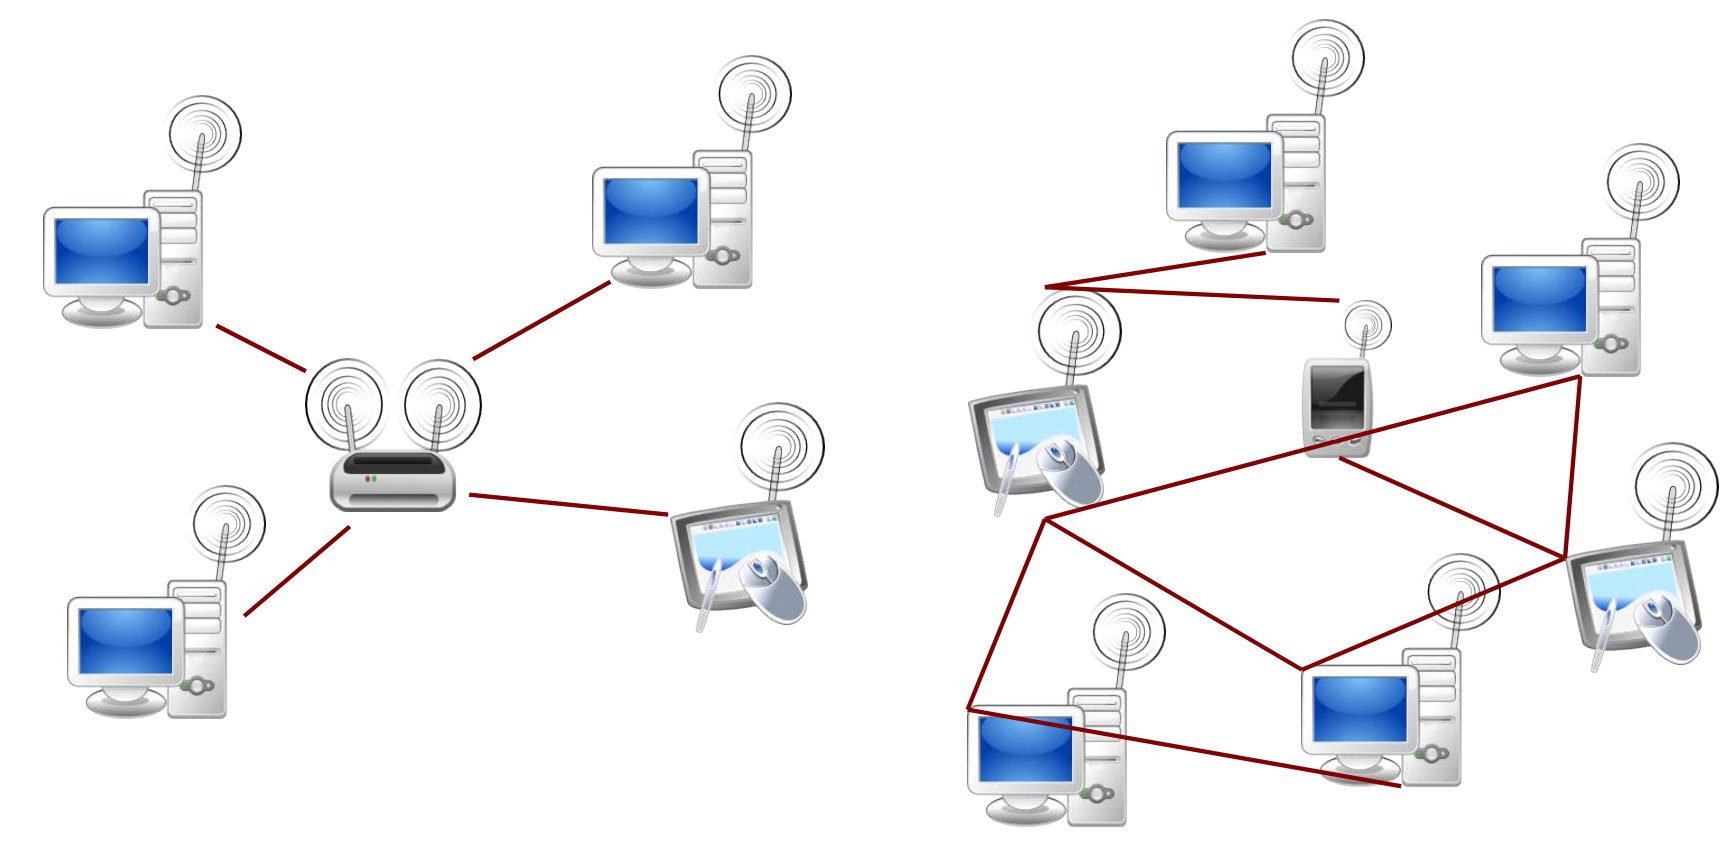
\includegraphics[scale = 0.4]{images/wireless-topology}
	\caption{Topologie reti wireless: centralizzata e distribuita.}
	\label{img:wireless-topology}
\end{figure}
In una rete centralizzata è necessario avere una mutua autenticazione tra host e AP centrale, mentre in una multi-hop tutti devono fidarsi di tutti quindi un attaccante può facilmente manipolare la rete una volta dentro.

La diffusione del Wi-Fi è dovuta principalmente alla sua semplicità di installazione, all'assenza di cavi ed alla comodità. Nelle reti Wi-Fi la banda utilizzabile effettivamente è una piccola percentuale rispetto al bitrate massimo: ad esempio nell'802.11b si ha un bitrate massimo di 5 Mb/s che è molto inferiore rispetto a quello massimo ($\approx$ 10 Mb/s). Il vantaggio principale di una rete ad-hoc è il multi-hop; lo scopo di queste reti è quello di essere del tutto auto-organizzanti ed estendibili.

Il fatto che per le reti wireless vi sia una mancanza di un limite geografico implica che le informazioni possono essere \textit{sniffate} più facilmente e si possono subire attacchi dall'esterno, dunque il rischio per l'attaccante è minimo. Vi è inoltre una ridefinizione del ruolo del livello MAC: l'accesso è inteso anche come \textquotedblleft controllo degli accessi"; a questo si aggiunge una maggior complessità dei firmware e dei driver. Si tenga comunque presente che abbiamo a che fare con dispositivi aventi risorse computazionali limitate.

Gli \textit{hotspot} sono punti di accesso ad internet che utilizzano la tecnologia wireless (normalmente 802.11) in modalità infrastructure. I vantaggi sono molteplici, ad esempio: abbattimento dei costi di gestione (non c'è cablaggio) ed installazione immediata. Vengono comunemente utilizzati in aeroporti, stazioni e alberghi. I problemi relativi alla gestione sono principalmente la limitazione del raggio e degli accessi.

Le reti \textit{ad-hoc/mesh} sono reti \textit{spontanee}, auto-organizzanti. Vengono principalmente utilizzate per ritrovi temporanei, riunioni, interventi in situazioni di emergenza, reti tattiche militari, ambienti con mancanza di infrastruttura (montagna, fiera), per sopperire al problema dell'ultimo miglio e per coprire aree molto estese.

Le reti \textit{PAN (Personal Area Network)} (dette anche Low-Power) sono reti di dimensioni ridotte utilizzate per interconnettere apparati (stampanti, computer, cellulari), configurate normalmente in modalità ad-hoc senza routing. Queste reti presentano un bitrate molto basso ed un raggio di copertura che può variare molto. La tecnologia più evoluta è lo standard Bluetooth, adesso confluito nell'IEEE 802.15.

Per quanto riguarda la \textit{legislazione}, le reti 802.11 b/g lavorano in frequenze non regolate (2.4 GHz, banda ISM -- Industrial, Scientific, Medical), quindi non sono soggette a licenza. Per queste frequenze in Italia il limite di potenza trasmissibile è di 100 mW per metro quadro, che permette comunicazioni in spazio libero fino a circa 300 metri con tecnologia 802.11. Le leggi ed i decreti presenti in Italia regolamentano l'utilizzo delle delle frequenze ISM e le modalità di autenticazione rendendone molto complicato l'utilizzo su suolo pubblico: questo ha frenato decisamente la diffusione di tali tecnologie sul suolo pubblico rispetto ad altri paesi (in cui vi sono regolamentazioni diverse). Lo svantaggio di ISM è la concentrazione di device che porta a collisioni continue.

La tecnologia \textit{WiMax} utilizza invece frequenze non in banda ISM. WiMax è una tecnologia nata per sostituire le connessioni cablate, che vanno dalla centrale del gestore alle singole abitazioni, anche connettendo tra loro più hotspot 802.11. Gli standard di riferimento sono l'IEEE 802.16d del 2004, e l'IEEE 802.16e del 2005. WiMax può utilizzare uno spettro di frequenze molto largo ($[2, 66]$ GHz), permette teoricamente collegamenti con un bitrate fino a 74 Mbps e può essere utilizzato anche su distanze molto grandi (chilometri). Una delle sue caratteristiche più importanti è quella di offre il controllo della qualità del servizio a livello MAC, oltre ad offrire anche una modalità ad-hoc (mesh). Era pertanto una tecnologia con delle grandi potenzialità, sopperita però perché rappresentava \textquotedblleft minacce" per i gestori telefonici, quindi per motivi prettamente commerciali.

La tecnologia \textit{bluetooth} è utilizzata per reti di piccole dimensioni, utilizzate per connettere tra di loro apparati dati (inizialmente auricolari, poi cellulari, stampanti, $\dots$). Opera in frequenze di 2.4 GHz, il suo bitrate massimo è 720 kbps per le versioni 1.1 e 1.2 e funziona normalmente in modalità ad-hoc (la versione 5 attuale supporta fino a 4 Mbit/s). Per quanto riguarda le distanze vi sono tre categorie di potenza, che permettono un raggio di copertura che varia dai 10 ai 100 metri. Sostanzialmente bluetooth è uno standard che funziona bene solo \textquotedblleft su carta", in realtà non offre grandi prestazioni ed è molto difficile da utilizzare perché il proprio standard si è evoluto \textquotedblleft a pezzi"; si è sviluppato cioè nel corso degli anni per offrire nuovi servizi (e al tempo stesso essere retrocompatibile): questo ha reso lo standard molto complesso. Oggi è utilizzato addirittura per lo stack protocollare TCP/IP: questo standard è nato semplicemente per far comunicare un telefono con un auricolare. Attualmente, al contrario di quando fu ideato, lo standard bluetooth non può più essere considerato PAN in senso stretto.

Altre tecnologie wireless sono: \textit{hyperlan2}, uno standard ETSI per reti locali wireless, con caratteristiche molto simili all'802.11, in realtà mai sviluppato e sopperito fin dall'inizio, e \textit{reti cellulari} come GSM, GPRS, UMTS $\dots$

Le reti, in generale, sono di tipo \textit{monoservizio} e \textit{multiservizio}. Le prime sono progettate per fornire un solo servizio all'utente (e.g. GSM, telegrafo, telefonia classica, Internet (nasce per trasmettere dati)). Le seconde, dette anche \textit{reti integrate nei servizi}, sono progettate per fornire più servizi agli utenti (e.g. ISDN e broadband ISDN -- oramai non più utilizzate); questo tipo di rete non ha mai avuto un grande successo per il semplice motivo che, essendo complesse, per il loro sviluppo servono diversi anni, dunque l'analisi dei requisiti effettuata in un primo momento del progetto non corrisponderà più alle esigenze che si vogliono soddisfare nel momento in cui questa diventa disponibile ed utilizzabile.

\section{Il protocollo 802.11 e Wi-Fi}
La prima versione dello standard 802.11, con la definizione dello strato MAC e delle caratteristiche di sicurezza, fu rilasciata nel 1996; il bitrate massimo era 2 Mbps. Nel 1999 furono sviluppate le versioni 802.11b, con un bitrate massimo di 11 Mbps, e 802.11a, versione per frequenze di 5 GHz con un bitrate massimo di 54 Mbps. Nel 2004, invece, furono sviluppate le versioni 802.11g, per frequenze di 2.4 GHz con bitrate massimo 54 Mbps, e 802.11i contenente una completa ristrutturazione dello strato di sicurezza. Nel 2007 venne introdotta la versione 802.11n, una versione con tecnologia MIMO (multiple-input multiple-output) che supporta bitrate superiori a 54 Mbps.

Il range di frequenze dell'802.11 è $[2.4, 5]$ GHz, il bitrate è circa $[11, 108]$ Mbps effettivi. Il raggio di copertura arriva fino a 50m in ambienti indoor e fino a 300m in ambienti outdoor senza linea di vista, e permette la mobilità.

La differenza sostanziale tra l'802.11 ed il WiFi è che il primo è un insieme di standard creati dalla IEEE per implementare reti wireless locali e si occupa del livelli 1 e 2, mentre il secondo è un trademark creato dalla Wifi-Alliance che certifica se un determinato dispositivo è conforme agli standard dell'802.11.

Prima che gli standard 802.11 vengano rilasciati ufficialmente, i maggiori produttori, che formano un consorzio WiFi (detto WiFi Alliance), rilasciano una pre-release e certificazioni sui prodotti hardware. In particolare, il consorzio, per rimediare all'emergenza causata dalle insicurezze riscontrate in tutte le versioni dell'802.11 precedenti alla $i$, anticipa nei propri prodotti una versione incompleta di 802.11i che chiama WPA (Wireless Protected Access). A questa segue WPA2, che corrisponde alla versione aderente a 802.11i. Attualmente esistono molti working group ($j,h,f,\dots$) con lo scopo di arricchire il protocollo con nuove caratteristiche quali QoS, fast handoff, etc. Negli standard vi è quindi sempre una parte resa volutamente \textit{implementation dependent}, che ha lo scopo di lasciare parti dello standard libere, in modo che le aziende possano scegliere quali parti dello standard utilizzare o personalizzare e quali no. Questa parte serve sostanzialmente per permettere la competizione tra aziende. Di seguito verrà introdotto il funzionamento di 802.11 nelle versioni precedenti alla $i$.\\
Nell'802.11 i pacchetti possono essere di tre tipi:
\begin{itemize}
	\item \textbf{Management}. Sono tutti i pacchetti che non trasportano dati, ma che vengono utilizzati dalle macchine per gestire il traffico dati. Questi includono pacchetti di autenticazione e deautenticazione, pacchetti di associazione e deassociazione, pacchetti di Beacon (pacchetti inviati continuamente dallo strato fisico contenenti il nome della rete (SSID), vedremo meglio in seguito). I pacchetti di management non prevedono nessuna forma di autenticazione o di cifratura. Il fatto che i pacchetti di autenticazione/deautenticazione non siano cifrati rappresenta una vulnerabilità dello standard (by design).
	\item \textbf{Control}. Sono tutti i pacchetti che non trasportano dati ma che vengono utilizzati dalle macchine per gestire l'accesso al canale, che avviene normalmente con politiche CSMA/CA. Vi sono quindi pacchetti di RTS/CTS (per risolvere il problema del terminale nascosto), di ACK, etc. Anche i pacchetti di controllo non prevedono nessuna forma di autenticazione o cifratura. Dal momento che i pacchetti di CTS non sono autenticati, un attaccante potrebbe pensare di mandare continuamente questi pacchetti in modo da saturare la banda e bloccare la rete.
	\item \textbf{Data}. Sono tutti i pacchetti che trasportano il contenuto informativo. Questi pacchetti possono essere cifrati ed autenticati.
\end{itemize}
Il \textbf{WEP} (Wired Equivalent Privacy) è l'insieme delle procedure introdotte in 802.11 per garantire privacy e sicurezza nelle comunicazioni, oltre al controllo degli accessi. Lo scopo dichiarato è quello di fornire un livello di sicurezza equivalente a quello di una rete cablata tradizionale. Le macchine appartenenti alla rete hanno tutte una chiave in comune, detta chiave WEP. Il WEP, in particolare, prevede:
\begin{itemize}
	\item Una \textit{unica chiave condivisa} tra tutte le macchine della rete per cifrare il traffico unicast e broadcast. Con questa strategia non esiste un'autenticazione dei pacchetti relativa alla singola macchina (non si sa chi ha effettuato l'accesso), non esistono comunicazioni segrete tra due singole macchine, non esiste un meccanismo automatico di \textit{refresh} della chiave ed un eventuale sniffing dei dati da parte di altri membri della rete è molto semplice.
	\item Una \textit{fase di autenticazione} in cui una nuova macchina dimostra di possedere la chiave. L'autenticazione è di tipo \textit{shared key}: il client si deve autenticare verso l'access point dimostrando di possedere la chiave segreta. Si noti che in sistemi più robusti (come WPA) la cifratura delle informazioni non è basata sulla chiave condivisa: questa viene infatti usata solamente per negoziare un'altra chiave che servirà a cifrare i dati. Quindi:
	\begin{enumerate}
		\item Il client chiede all'AP di autenticarsi.
		\item L'AP risponde con un \textit{challenge text}.
		\item Il client risponde con il \textit{challenge text cifrato}.
	\end{enumerate}
	Questa idea non è molto buona: un attaccante potrebbe intercettare challenge in chiaro e challenge cifrato da cui è possibile risalire alla chiave.\\
	In questa fase i pacchetti sono di tipo management, dunque non sono né autenticati né cifrarti. In pratica viene cifrato solo il campo di payload del pacchetto, con un algoritmo di cifratura di tipo stream. La procedura è molto veloce e quindi pensata per poter essere utilizzata come procedura di handoff rapido anche tra più AP. L'AP in questo caso è l'unico elemento che decide chi far entrare nella rete: la gestione degli accessi è quindi tutta sull'AP stesso. Per reti costituite da più AP la gestione diventa molto complessa o del tutto statica.
	\item Un \textit{algoritmo di cifratura} dei pacchetti di tipo \textit{stream}, l'RC4, che tuttavia è un algoritmo estremamente debole.
\end{itemize}
Gli algoritmi \textit{stream} cifrano il payload in chiaro bit per bit, e non a blocchi di dimensione fissa. In pratica, a partire da un segreto, si genera un vettore di lunghezza variabile di dati pseudocasuali (\textit{keystream}). Per rendere unico ogni pacchetto si aggiunge al segreto un vettore di inizializzazione (IV), dunque il keystream dipende dalla coppia (segreto, IV). Si effettua infine uno XOR logico tra il keystream e l'informazione da cifrare. Uno schema logico dell'algoritmo è riportato in Figura \ref{graph:stream-encryption}.\\
Gli algoritmi di tipo stream sono molto veloci e facili da implementare; riutilizzare più volte lo stesso IV significa ripetere due volte lo stesso keystream, dunque se si è a conoscenza di uno dei due pacchetti in chiaro è possibile ricavare anche il secondo. Dunque, lo stesso keystream non deve essere mai utilizzato.
\begin{figure}[htbp]
	\centering
	\begin{tikzpicture}[->,>=stealth',shorten >=1pt,auto,node distance=5.8cm,
	semithick, scale = 0.6, transform shape]
	
		\node[rect,align=center] (1) {Generatore di numeri\\pseudocasuali};
		\node[] (2) [left of=1] {($K$, IV)};
		\node[state] (3) [right of=1] {$+$};
		\node[] (4) [above of=3,yshift=-3cm] {Testo in chiaro};
		\node[] (5) [right of=3,xshift=-2cm] {Testo cifrato};
		
		\path (2) edge node {} (1)
		(1) edge node {Keystream} (3)
		(4) edge node {} (3)
		(3) edge node {} (5);
	\end{tikzpicture}
	\caption{Algoritmo di cifratura di tipo stream. Il simbolo \textquotedblleft $+$" rappresenta l'operatore logico XOR.}
	\label{graph:stream-encryption}
\end{figure}\\
Vediamo adesso la procedura di cifratura con RC4 (Figura \ref{img:RC4-encryption}):
\begin{figure}[htbp]
	\centering
	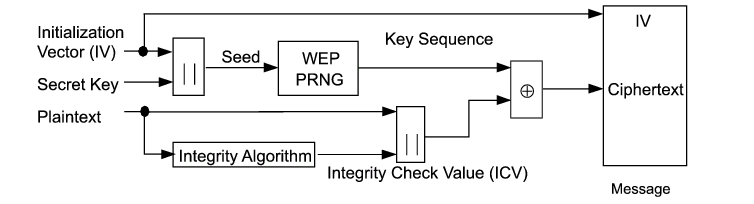
\includegraphics[scale = 0.5]{images/RC4-encryption}
	\caption{Procedura di encryption con RC4.}
	\label{img:RC4-encryption}
\end{figure}
\begin{enumerate}
	\item Si concatena la chiave WEP con il IV per generare il \textit{seed}.
	\item Il blocco WEP PRNG (Pseudo Random Number Generator, basato su RC4) genera un \textit{keystream} a partire dal \textit{seed}.
	\item Sul \textit{plaintext} (testo in chiaro) si applica un algoritmo di \textit{error detection} (CRC-32) ed il CRC viene concatenato al pacchetto in chiaro.
	\item Si effettua uno XOR con la chiave.
	\item Si trasmette il pacchetto con l'IV nell'header (non cifrato) ed il payload cifrato.
\end{enumerate}
RC4 utilizza in 802.11b chiavi a 40 bit. In generale un buon (pseudo) random generator è un algoritmo che, a partire dal seed, ad ogni passo genera uno o più numeri nel modo più impredicibile possibile, dovrebbe avvicinarsi cioè al \textit{rumore bianco}. Si noti che l'impredicibilità assoluta è impossibile. Vediamo dunque la procedura di decifratura (Figura \ref{img:RC4-decryption}):
\begin{figure}[htbp]
	\centering
	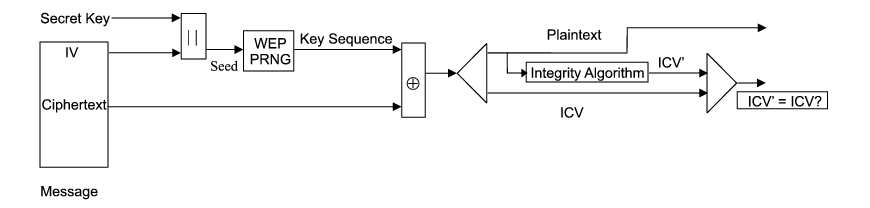
\includegraphics[scale = 0.5]{images/RC4-decryption}
	\caption{Procedura di decryption con RC4.}
	\label{img:RC4-decryption}
\end{figure}
\begin{enumerate}
	\item Dal pacchetto si estrae l'IV ed il payload cifrato.
	\item Dall'IV e dalla chiave WEP si ricrea il \textit{keystream}.
	\item Si effettua uno XOR tra il \textit{keystream} ed il payload ottenendo il payload in chiaro.
	\item Si separa il payload dal CRC e si ricalcola il CRC per verificare l'integrità.
\end{enumerate}
Cifrare anche il CRC significa che se un attaccante non conosce la chiave di cifratura può modificare il pacchetto, ma non può rendere coerente il CRC. Così facendo si ottiene la sicurezza dell'integrità delle informazioni. Vediamo quindi come viene effettuata l'\textit{autenticazione dei frame}:
\begin{enumerate}
	\item Si calcola il CRC sul payload in chiaro.
	\item Si concatena il CRC al payload in chiaro e si effettua uno XOR tra il \textit{keystream} ed il payload ottenendo il payload cifrato.
	\item Si trasmette il pacchetto (header in chiaro, payload cifrato).
	\item Una volta ricevuto il pacchetto, si estrae l'IV dall'header e si utilizza per ricalcolare il \textit{keystream} (attraverso la chiave WEP); si esegue uno XOR con il pacchetto e si ricava il payload in chiaro concatenato al CRC.
	\item A questo punto si ricalcola il CRC dal payload in chiaro e si confronta con quello ricevuto. Se i due valori coincidono, la trasmissione è avvenuta senza manomissioni.
\end{enumerate}
Così facendo otteniamo un controllo di integrità sul payload.

Facciamo adesso alcune precisazioni e note sul WEP. (a) L'autenticazione dei pacchetti non utilizza algoritmi a chiave pubblica/privata; dovrebbe invece esserci sempre un segreto condiviso in precedenza, dunque un canale sicuro. (b) Alcuni AP implementano un filtro sugli indirizzi MAC da far accedere alla rete per evitare accessi indesiderati. (c) Non esiste controllo di unicità dei pacchetti, due pacchetti possono essere identici. (d) Non esiste controllo di sequenza dei pacchetti, il valore di IV viene deciso dagli apparati senza una politica definita (e.g. randomica, incrementale, $\dots$). Un attaccante può ripetere un pacchetto anche senza conoscerne il significato: i protocolli di livello superiore hanno il compito di gestire i dati, accettandoli o rifiutandoli.

Vediamo ora nel dettaglio l'ingresso e l'uscita dalla rete (cfr. macchina a stati in Figura \ref{img:802_11-state-machine}). Per quanto riguarda l'\textit{associazione} (richiesta di voler dialogare con l'AP), una volta autenticato, il client deve notificare all'access point che vuole entrare nella rete; questo avviene semplicemente in due fasi: (1) Il client chiede di associarsi, (2) L'access point invia una conferma. Per quanto riguarda, invece, l'uscita dalla rete sono previste le fasi di \textit{deautenticazione} e \textit{deassociazione}; per deautenticare il client, l'AP invia un messaggio di deautenticazione ed il client deve ripetere l'autenticazione, mentre per deassociare un client, l'AP invia un messaggio di deassociazione e il client deve ripetere l'associazione. Se il client riceve un messaggio di deautenticazione quando è anche associato, allora dovrà ripetere entrambe le fasi. Si noti che questi sono tutti pacchetti di management.
\begin{figure}[htbp]
	\centering
	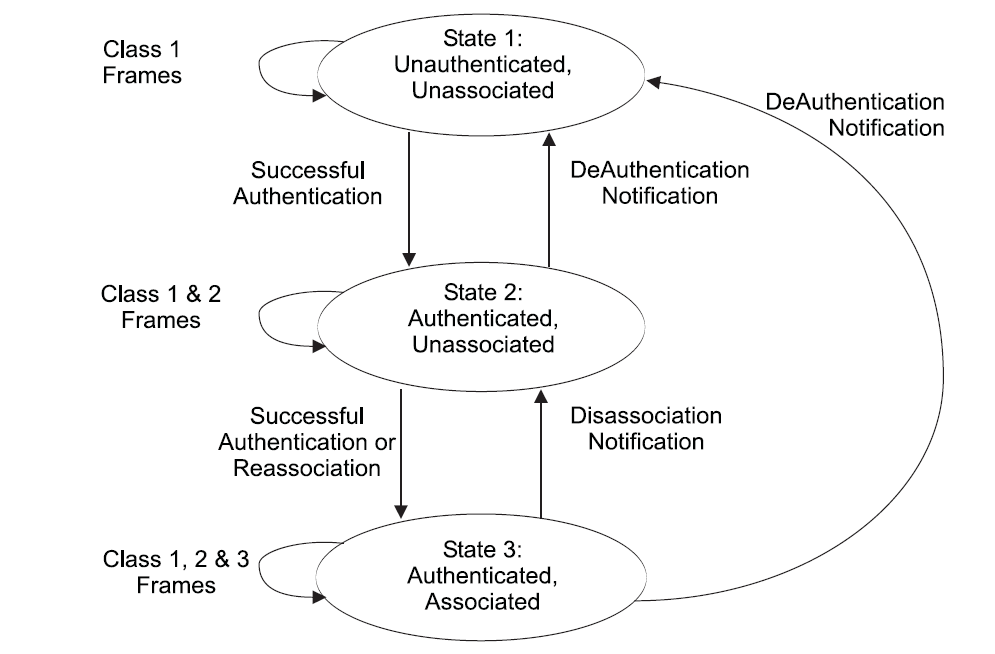
\includegraphics[scale = 0.3]{images/802_11-state-machine}
	\caption{Macchina a stati per l'ingresso e l'uscita dalla rete del protocollo 802.11.}
	\label{img:802_11-state-machine}
\end{figure}\\
Per quanto riguarda la tecnica di \textit{accesso al canale}, l'802.11 prevede che i client della WLAN condividano lo stesso canale fisico con una politica di accesso CSMA/CA. In modalità infrastructure, l'AP si comporta da centro stella, dunque tutto il traffico viene inviato all'AP che, a sua volta, lo redirige verso ai client. Nell'intestazione di ogni pacchetti ACK/RTS è presente un campo \textit{duration} in cui il client specifica un periodo di tempo durante il quale il canale è prenotato: in tale periodo il canale non viene utilizzato da altri client. Un problema molto noto di questo tipo di accesso è il \textit{problema del terminale nascosto}. Si consideri la situazione rappresentata in Figura \ref{img:hidden-node-problem}.
\begin{figure}[htbp]
	\centering
	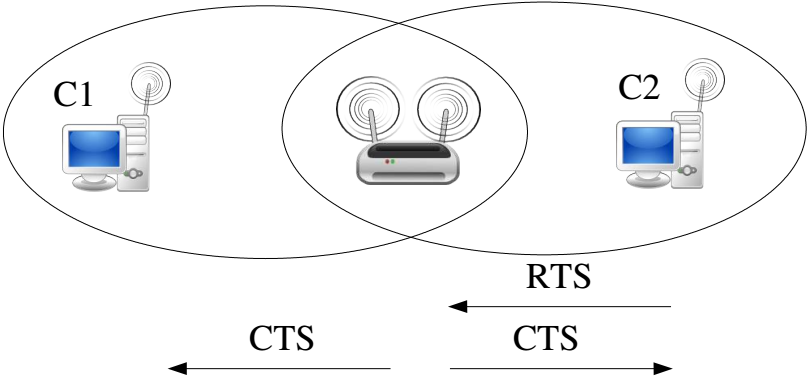
\includegraphics[scale = 0.5]{images/hidden-node-problem}
	\caption{Problema del terminale nascosto.}
	\label{img:hidden-node-problem}
\end{figure}\\
Le ellissi rappresentano le aree di copertura tra l'AP ed i client $C_1$ e $C_2$. In sostanza, l'AP può comunicare con entrambi i client $C_1$ e $C_2$, ma qualcosa (ad esempio la distanza) impedisce a $C_1$ e $C_2$ di comunicare direttamente tra loro e quindi anche di poter rilevare (\textit{sensing}) la portante trasmessa dall'altro client verso l'AP. In questo contesto è allora possibile che si verifichino collisioni in ricezione sull'AP quando entrambi i client $C_1$ e $C_2$, rilevando il canale libero, trasmettono contemporaneamente verso l'AP. Per evitare collisioni, lo standard IEEE 802.11 permette di usare un meccanismo con il quale la stazione, prima di inviare un frame, richiede la trasmissione di speciali piccoli pacchetti:
\begin{itemize}
	\item \textbf{RTS} (Request To Send): oltre a riservarsi il mezzo, fa tacere qualsiasi stazione che lo sente.
	\item \textbf{CTS} (Clear To Send): viene inviato dall'AP in risposta all'RTS, e ha il compito di far tacere le stazioni nell'immediata vicinanza.
\end{itemize}
Dunque, se ad esempio $C_1$ vuole trasmettere all'AP, invia un messaggio RTS. Se l'AP non sta comunicando con nessun altro nodo, allora invia un messaggio CTS in cui dà il permesso a $C_1$ di trasmettere, ed a tutti gli altri nodi (nel caso in Figura \ref{img:hidden-node-problem} solo $C_2$) indica che in quel momento sta effettuando una comunicazione con un altro nodo.
\begin{figure}[htbp]
	\centering
	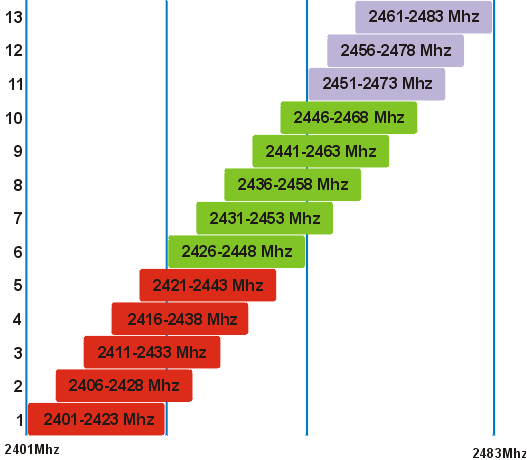
\includegraphics[scale = 0.4]{images/802_11-channels}
	\caption{Canali del protocollo 802.11.}
	\label{img:802_11-channels}
\end{figure}\\
A scopo informativo, in Figura \ref{img:802_11-channels} sono riportate le bande di frequenza dei 13 canali sulle quali lavora il protocollo 802.11. Notiamo che vi sono parziali sovrapposizioni tra i canali (in termini di frequenze fuori dal centrobanda) e queste possono causare dei disturbi. In pratica, anche se viene utilizzato soltanto il centrobanda, è impossibile realizzare dei filtri passabanda che taglino precisamente un intervallo di frequenze (cioè dei filtri ideali); allontanandosi dal centrobanda, quindi, il segnale è attenuato progressivamente ma non è esattamente nullo. Questo problema viene risolto semplicemente utilizzando canali che non presentano overlap, ad esempio 1, 6 e 11.

Facciamo adesso una precisazione sui beacon frame. Il beacon è un pacchetto che viene inviato dagli AP per segnalare la propria presenza. I contenuti più importanti del Beacon Frame sono: la \textit{modalità} (ad-hoc o infrastructure), \textit{ESSID} (cioè il nome dell'AP; è necessario specificarlo per entrare nella rete durante la fase dell'associazione) e \textit{privacy} (definisce se l'AP supporta WEP o meno). Allo stato attuale le reti ad-hoc sono poco utilizzate.

Il WDS (Wireless Distribution System) è un sistema di scambio di dati tra AP. Quando gli APs vogliono fare routing dei pacchetti tra di loro, per unire due reti distinte fisicamente in una unica rete logica devono utilizzare le interfacce WDS. Sulle interfacce WDS si può utilizzare WEP, ma non esiste associazione o autenticazione. L'utilizzo di interfacce WDS tuttavia sottrae banda per il servizio della rete infrastructure.

\section{Insicurezze del protocollo 802.11}
Le insicurezze che vedremo sono relative al protocollo 802.11 nelle versioni a/b/g. Alcune di queste non riguardano gli algoritmi crittografici utilizzati, quindi si ritrovano anche nella versione 802.11i.

Gli attacchi \textit{Denial of Service} (DoS) sono attacchi mirati all'interruzione dell'erogazione del servizio. Se il servizio è l'accesso stesso Internet (ad esempio un hotspot che offre connettività), il danno in termini economici è rilevante; esistono infatti situazioni Mission Critical in cui non è possibile permettersi di non avere connettività (e.g. scadenze produttive, reti di emergenza, etc.) e l'interruzione del servizio rende all'utente una generale impressione di inaffidabilità, dunque lo allontana. Le reti Wi-Fi in generale non dovrebbero essere usate in situazioni Mission Critical.\\
Abbiamo già visto come avviene l'autenticazione di un host verso l'AP: il client chiede di autenticarsi, l'AP risponde con un challenge text ed infine il client risponde con il challenge text cifrato. I pacchetti di autenticazione non sono a loro volta autenticati, dunque un attaccante potrebbe falsificarli. In particolare, durante la fase di ingresso, l'attaccante attende l'autenticazione e risponde al posto dell'AP con un pacchetto di deautenticazione. In questo modo può evitare che le macchine entrino in rete ed in qualsiasi momento l'attaccante può inviare un pacchetto per forzare l'uscita dalla rete di un client. Gli scopi possono essere molteplici; ad esempio è possibile evitare che un determinato client si connetta o semplicemente è possibile tenere fuori dalla rete altri client per avere più banda. Tuttavia, se l'attaccante vuole continuare a produrre l'attacco deve continuamente stare in ascolto di nuove autenticazioni.\\
Lo stesso tipo di attacco può essere effettuato sull'associazione (cfr. Figura \ref{img:802_11-state-machine}); la differenza sta nel fatto che questo attacco non richiede una riautenticazione, quindi ha meno impatto. Può servire ad esempio a far rivelare l'ESSID ad un AP che non lo vuole mostrare.\\
Questi due tipi di attacco sono ancora più pericolosi se l'attaccante, oltre a cambiare l'indirizzo sorgente (\textit{spoofing}), utilizza l'indirizzo destinazione di broadcast. Alcuni client sono configurabili per non accettare le richieste di deautenticazione/deassociazione in broadcast, non rispettando tuttavia lo standard.
\begin{figure}[htbp]
	\centering
	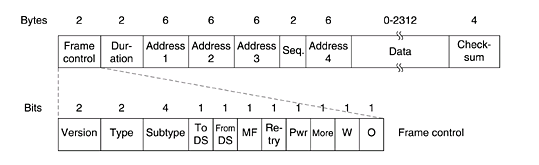
\includegraphics[scale = 0.8]{images/802_11-frame}
	\caption{Formato generico del frame 802.11 e formato del campo \textit{framecontrol}.}
	\label{img:802_11-frame}
\end{figure}\\
Un altro tipo di attacco DoS è quello sull'\textit{accesso al canale}. Si consideri il formato del generico frame 802.11 riportato in Figura \ref{img:802_11-frame}. Il campo \textit{duration} (espresso in $\mu s$) specifica il tempo per cui il canale rimarrà occupato dal mittente del pacchetto; ogni macchina della rete che riceve un pacchetto qualsiasi, anche se non è rivolto al proprio indirizzo MAC, deve leggere e rispettare il campo \textit{duration}. Un attaccante potrebbe inviare un nuovo pacchetto prima che scada il timeout, prenotando nuovamente il canale. In questo modo nessuna macchina, esclusa quella dell'attaccante, può trasmettere. Sostanzialmente questo è un errore di progettazione del protocollo: l'informazione \textit{duration} dovrebbe essere inviata separatamente dalle altre presente nel frame.\\
Il quarto tipo di attacco DoS che prendiamo in considerazione è quello sulla \textit{modalità Power Save}. Consideriamo il formato del campo \textit{framecontrol} riportato in Figura \ref{img:802_11-frame}. Il bit Power Save (Pwr) viene utilizzato dal client per segnalare all'AP che sta entrando in modalità power save. In modalità power save l'AP non trasmette il traffico al client (ma può ricevere): i frames sono salvati in un buffer e vengono trasmessi a burst quando il client li richiede. Un attaccante potrebbe inviare, con una certa frequenza, pacchetti modificati con il bit power save $\text{Pwr} = 1$ (\textit{spoofing}). In questo modo l'AP non trasmetterà mai i frames memorizzati nel buffer. Il risultato è un DoS che isola una singola macchina della rete senza uno sforzo notevole da parte dell'attaccante.\\
Il quinto tipo di attacco DoS è quello che causa una \textit{saturazione} della banda. Per individuare le macchine circostanti vengono utilizzati dei \textit{probe} (pacchetti simili a quelli del ping, ma di livello 2): la macchina richiedente invia all'indirizzo di broadcast un messaggio di management di tipo \textit{probe request} e tutte le macchine che ricevono la richiesta rispondono con un \textit{probe reply} diretto al richiedente. I messaggi di probe, essendo messaggi di management, non vengono cifrati, dunque l'attaccante potrebbe falsificarli provocando risposte dagli altri host della rete. Ripetendo continuamente le richieste è possibile occupare tutta la banda disponibile sfruttando l'effetto di riflessione degli altri host. Al contrario del DoS sulla deautenticazione, in questo caso gli host non possono evitare di rispondere ai messaggi di probe in broadcast, perché verrebbe annullata l'utilità stessa del meccanismo di probing.\\
Il sesto (ed ultimo) tipo di attacco DoS viene effettuato a livello fisico: il \textit{jamming}. Il protocollo 802.11 utilizza una codifica \textit{spread spectrum}, in cui il segnale viene trasmesso utilizzando una banda più larga di quanto non sarebbe necessario, aggiungendo ridondanza; a destinazione il segnale viene ricostruito in una gamma più stretta. In questo modo un segnale molto potente, ma concentrato su una gamma di frequenze molto ristretta, viene ricevuto a destinazione (dopo la ricostruzione) come un rumore distribuito su tutta la banda. È quindi molto difficile riuscire a disturbare la ricezione di tutti i dati. Nonostante questo è molto importante notare che i pacchetti del protocollo 802.11 hanno un codice di controllo degli errori (Figura \ref{img:802_11-frame}). Dunque, anche se è difficile disturbare la ricezione di un intero pacchetto, se si riesce a disturbare la ricezione di un solo bit, che statisticamente è un risultato più accessibile, si provoca il fallimento del controllo di errore ed il pacchetto viene scartato, quindi deve essere trasmesso di nuovo.

Un altro tipo di attacco è quello che mira ai \textit{software degli AP}; vediamo due esempi. Spesso gli AP presentano interfacce web per la gestione. Le macchine collegate alla rete possono accedere all'interfaccia di gestione, da cui è possibile configurare gli AP. Si è verificato spesso che queste interfacce presentassero delle vulnerabilità come \textit{buffer overflow} o password attive di default che permettessero anche agli utenti della rete senza password di amministrazione di modificare delle configurazioni. A volte un reset improvviso degli AP potrebbe provocare un riavvio in una modalità provvisoria che offre anche ad utenti senza credenziali di accedere all'interfaccia di gestione.\\
Un altro esempio sfrutta un bug dei software degli AP. Gli AP devono mantenere una lista delle macchine autenticate nella rete, delle macchine associate e delle macchine che hanno richiesto l'autenticazione ma che ancora non hanno completato le procedure. Quando una lista si riempie, le altre richieste in arrivo vengono scartate. Per la gestione di queste liste devono essere applicate politiche efficienti; alcuni esempi di inefficienza sono i seguenti:
\begin{itemize}
	\item Le liste sono delle code a scorrimento: se la lista è piena e arriva una nuova macchina, la più vecchia viene tolta dalla lista. Forgiando richieste di autenticazione false si riempie la lista e si impediscono anche le autenticazioni già in corso.
	\item Le tre liste sono unite in una sola lista. Questa inefficienza ha un effetto peggiore rispetto a quello del difetto precedente.
	\item Non avviene una corretta gestione della memoria per le liste. Si può pertanto produrre un buffer overflow, provocando il blocco o il riavvio dell'AP.
\end{itemize}
Esistono molti esempi di \textit{exploit} su AP derivanti da bug di questo tipo.

Un ulteriore aspetto relativo alle insicurezze del protocollo 802.11 è l'\textit{autenticazione con shared key}. Come già detto, la chiave è unica ed in questo modo non esiste alcuna segretezza, dunque autenticazione tra macchine della stessa rete. Una macchina autenticata può spostare la chiave su altre macchine e lasciare che queste entrino. Anche le Access List sugli AP (che non fanno parte dello standard) sono generalmente statiche, quindi il problema della gestione è importante. Inoltre, sulla maggior parte delle schede wireless, è possibile cambiare l'indirizzo MAC. Essendo quindi la chiave statica, tutta la fiducia è riposta nella certezza che l'algoritmo di autenticazione e cifratura sia robusto. Per lo stesso motivo l'AP non si autentica con le macchine.\\
L'autenticazione shared key è tragicamente insicura: nel giro di pochi secondi passa lo stesso testo (128 byte) prima in chiaro e poi cifrato. L'attaccante può recuperare un frammento di keystream che può utilizzare per inviare pacchetti nella rete (anche senza possedere la chiave WEP), può effettuare un attacco di tipo reply anche senza conoscere la chiave (spacciandosi per l'AP) e può effettuare il cosiddetto \textit{attacco dell'oracolo} (\textit{oracle attack}). Lo scopo di questo attacco è quello di inviare un messaggio nella rete senza conoscere la chiave segreta. In pratica in un primo momento l'attaccante provvede a deautenticare un client; successivamente forgia un pacchetto con un challenge text contenente i dati che vuole inviare in rete ed a questo punto il client risponde restituendo il challenge text cifrato con un certo IV, ovvero il pacchetto valido, pronto per essere inviato lungo massimo 128 byte. L'attacco può essere utilizzato verso un client, quando nella rete non avviene autenticazione shared key, per ricavare un frammento di keystream. Una volta conosciuta una parte del keystream (128 byte) vi è la necessità di aggiungere altre informazioni al pacchetto affinché questo risulti completo. Il challenge text non può essere allungato perché la parte di autenticazione prevede 128 byte. L'idea è quindi quella di aggiungere poche informazioni alla volta e provare ad inviare il pacchetto osservando la risposta. Si effettuano dunque delle richieste a lunghezza variabile a cui gli host sono costretti a rispondere, come ad esempio il ping. Questo attacco non ha tuttavia un utilizzo concreto molto comune, ma dimostra la goffaggine con cui sono stati progettati i meccanismi di sicurezza del protocollo.\\
Questi problemi hanno spinto i produttori di AP e i gestori delle reti a preferire come scelta di default l'autenticazione open-system, ovvero senza alcuna forma di autenticazione. Per evitare che chiunque entri nella rete si preferisce mascherare nei beacon l'ESSID dell'AP che è un parametro necessario per richiedere l'associazione, ma in questo modo si crea un'altra divergenza dallo standard.

Un altro attacco possibile è quello di tipo \textit{Man-In-The-Middle} (MITM). In questo caso per attacco MITM si intende la possibilità di convogliare tutto il traffico tra due host attraverso l'attaccante con molteplici scopi tra cui:
\begin{itemize}
	\item assicurarsi che il traffico che si vuole intercettare passi per la propria macchina;
	\item convincere una macchina che la forma di autenticazione è cambiata e che adesso non si deve più utilizzare una chiave WEP;
	\item poter influenzare le procedure di autenticazione e crittografia degli strati superiori (e.g. attacco MITM sui certificati SSL).
\end{itemize}
Dunque prima dell'attacco si avrebbe una situazione in cui tutti i device sono collegati ad un AP (compreso quello dell'attaccante), mentre dopo l'attacco alcuni device risultano collegati a quello dell'attaccante (che è connesso comunque all'AP). In pratica qualsiasi macchina della rete che possiede la chiave WEP può spacciarsi per l'AP. Se l'attaccante deautentica un host, questo cercherà in un secondo momento di ripetere l'autenticazione. L'attaccante può pensare quindi di generare una \textit{race condition} per cui può cercare di rispondere prima dell'AP, eventualmente con l'aiuto di una seconda scheda con la quale produrre un attacco DoS sul vero AP in modo da favorirsi nella \textit{gara}. Spesso, dopo un certo numero di connessioni, un host cercherà di ripetere l'autenticazione su un canale diverso facendo \textit{channel hopping}. L'attaccante può mettersi in ascolto su un'altro canale: in questo modo è sicuro che la vittima si collegherà con lui. I finti AP si chiamano comunemente \textit{Rogue AP} o \textit{Fake AP}.

L'ultimo tipo di attacco che vediamo al protocollo 802.11 è quello agli \textit{algoritmi crittografici}. Abbiamo già detto che il WEP utilizza l'algoritmo crittografico RC4, la cui procedura di encryption è schematizzata in Figura \ref{img:RC4-decryption}. La non ripetizione degli IV è fondamentale per non rischiare di esporre il materiale cifrato: riutilizzare un IV, infatti, significherebbe utilizzare due volte lo stesso \textit{keystream}. Se si è a conoscenza del contenuto in chiaro di uno dei due pacchetti cifrati aventi \textit{keystream} uguale, automaticamente è possibile risalire al \textit{keystream} stesso e dunque al contenuto di tutti i pacchetti cifrati con lo stesso IV. È possibile costruire un dizionario di tutti i \textit{keystream}? Considerando che il campo IV è lungo 24 bit, si avrebbero 16 777 216 IV diversi; ogni pacchetto tipicamente è lungo 1500 byte (in realtà anche di più), quindi in totale, affinché un IV si ripeta, dovrebbero passare circa 25 GB di dati che, su una rete avente $\approx$ 30 Mbit/s di banda, si otterrebbero in circa due ore. Questo permette in linea teorica di poter costruire un dizionario di tutti i \textit{keystream}. Per ricavare un \textit{keystream} l'attaccante dovrebbe conoscere il contenuto del pacchetto cifrato che vede passare. Esistono dei pacchetti il cui contenuto è riconoscibile dalla propria lunghezza (e.g. DHCP request). Quando l'attaccante intercetta un pacchetto avente la lunghezza voluta, automaticamente conosce il contenuto, dunque ricava il \textit{keystream}. Se tuttavia la rete è poco popolata potrebbe essere necessario molto tempo affinché si intercetti il pacchetto desiderato.\\
Per trovare il keystream è sufficiente effettuare uno XOR tra il pacchetto con payload cifrato ed il pacchetto in chiaro (noto):
\begin{figure}[htbp]
	\centering
	\begin{tabular}{r}
		{\begin{bytefield}{24}\bitbox{8}{Header}\bitbox{16}{Payload cifrato}\end{bytefield}}\\
		$\bigoplus\hspace{2.5cm}$\\
		{\begin{bytefield}{16}\bitbox{16}{Pacchetto in chiaro (noto)}\end{bytefield}}\\
		$=\hspace{2.5cm}$\\
		{\begin{bytefield}{16}\bitbox{16}{Keystream}\end{bytefield}}\\
	\end{tabular}
\end{figure}\\
Vediamo adesso un metodo per estendere il keystream: il \textit{chopchop attack}. Il keystream ricavato non è lungo quando l'MTU della rete: l'attaccante in qualche modo deve poterlo estendere. Se si è a conoscenza di un keystream lungo $N$ bytes, è possibile forgiare un nuovo pacchetto (e.g. ping) avente dimensione $N+1$ bytes, ma non è possibile cifrare quest'ultimo byte aggiuntivo di keystream: si suppone inizialmente che sia 0$\times$00. L'attaccante ricalcola il CRC, lo accoda al pacchetto e lo invia. A destinazione il CRC viene verificato: se il byte non era 0$\times$00 il controllo fallisce e non viene ricevuta risposta, altrimenti, se viene ricevuta una risposta, 0$\times$00 era il byte giusto. Nel caso di mancata risposta si riprova con 0$\times$01 e così via. La situazione è riportata in modo schematico in Figura \ref{img:chopchop-attack}. Mediamente dopo 128 tentativi si ottiene il byte di estensione e per ottenere tutto un keystream senza impattare troppo sulla rete bastano 24 ore. Questo è un attacco di tipo \textit{attivo}.
\begin{figure}[htbp]
	\centering
	\begin{tabular}{r}
		{\begin{bytefield}{24}\bitbox{8}{Header}\bitbox{10}{Pacchetto Ping}\bitbox{2}{FF}\bitbox{4}{CRC}\end{bytefield}}\\
		$\bigoplus\hspace{2.5cm}$\\
		{\begin{bytefield}{16}\bitbox{14}{Keystream}\bitbox{2}{00}\end{bytefield}}\\
		$=\hspace{2.5cm}$\\
		{\begin{bytefield}{24}\bitbox{8}{Header}\bitbox{16}{Pacchetto cifrato}\end{bytefield}}\\
	\end{tabular}
	\caption{Attacco chopchop. Il valore FF è insignificante ai fini dello XOR: potrebbe esserci qualsiasi altro valore.}
	\label{img:chopchop-attack}
\end{figure}\\
A questo punto l'attaccante ha a disposizione un keystream intero e può quindi iniettare nella rete pacchetti che vengono elaborati correttamente dalle macchine della rete stessa. Esiste un'opzione del protocollo ICMP che impone ad una macchina che riceve un ping di rispondere esattamente con lo stesso pacchetto. L'attaccante può dunque forgiare dei ping di 1500 byte ed inviarli con certi IV, conoscendo a priori la risposta. La vittima risponderà utilizzando IV diversi, quindi mettendo a disposizione dell'attaccante nuovi keystream.\\
Per avere accesso non autorizzato ad una rete 802.11, pertanto, è necessario effettuare le seguenti operazioni:
\begin{enumerate}
	\item individuazione del pacchetto DHCP (attacco dell'oracolo) $\longrightarrow$ pochi secondi,
	\item estensione del keystream $\longrightarrow$ 24 ore,
	\item generazione del dizionario $\longrightarrow$ 3/4 ore,
\end{enumerate}
per un totale di circa 28 ore. Se non si vuole rendere l'attacco troppo evidente è necessario diminuire il traffico generato e raddoppiare (o triplicare) il tempo occorrente. Una volta costruito il dizionario si possono decifrare tutti i
pacchetti della rete, oltre inviarli senza conoscere la chiave segreta. Si noti che il tempo non varierebbe in funzione della velocità della rete (i tre tempi riportati sopra rimarrebbero circa uguali); inoltre, se la rete è poco popolata, potrebbe essere necessario molto tempo per svolgere la prima operazione.\\
Avendo a disposizione chiavi statiche, una vita media di 28 ore è troppo breve (andrebbe cambiata la chiave circa una volta al giorno). Si noti che è possibile costruire un dizionario perché la sequenza degli IV non è vincolata; come conseguenza alcuni produttori hanno allungato il campo IV non rispettando lo standard. Questa tuttavia non rappresenta assolutamente una soluzione al problema, in quanto provvede solo ad aumentare (di poco) il tempo di vita medio di una chiave.

Nel 2001 Fluhrer, Mantin e Shamir trovarono una vulnerabilità nel modo in cui RC4 genera i keystream. In particolare, quando si utilizzano determinati IV per generare il keystream esiste una correlazione statistica tra il primo byte del keystream e la chiave segreta utilizzata; in questo caso si dice che esistono IV \textit{deboli}. Raccogliendo almeno 60 pacchetti cifrati a partire da IV deboli \textit{è possibile ricavare la chiave segreta}. Si noti che non si parla come nel precedente caso di un keystream, ma della \textit{chiave segreta} che viene inserita nella cifratura WEP e che, una volta compromessa, dà accesso completo alla rete.\\
Gli IV deboli sono distribuiti uniformemente nello spazio degli IV e per ottenere i 60 IV di interesse sono necessari mediamente 4 milioni di pacchetti cifrati. Quindi, in dipendenza del traffico generato dalla rete, in poche ore è possibile rompere una chiave WEP ed ottenere quindi una chiave segreta a 40 bit. A differenza dell'attacco chopchop che abbiamo detto essere attivo, questo è un attacco \textit{passivo}, dunque difficile da rilevare: il rischio per un attaccante di essere scoperto è veramente basso. Per aumentare il tempo necessario a svolgere l'attacco si può pensare di rendere maggiore la dimensione della chiave; tuttavia la complessità dell'attacco aumenta \textit{linearmente} con la lunghezza della chiave WEP, quindi anche utilizzando chiave a 128, 256, $\dots$ bit il tempo necessario ad ottenere la chiave WEP aumenta linearmente e l'attacco è sempre valido e fattibile. In genere un aumento lineare della complessità non è esattamente ciò che dovremmo aspettarci da un buon algoritmo: la complessità dell'attacco dovrebbe aumentare in modo esponenziale o parabolico rispetto alla lunghezza della chiave. Per ovviare a questo problema alcuni produttori impediscono ai loro AP di utilizzare IV deboli, non rispettando però lo standard.\\
Nell'agosto del 2004 l'hacker $KoreK$ inviò su un forum un programma basato su una sua ricerca statistica che evidenziava l'esistenza di una correlazione anche tra altri byte del keystream e la chiave WEP, rendendo quindi l'attacco precedente ancora più facile. Successivamente vennero pubblicate nuove migliorie: per rompere una chiave WEP è sufficiente \textit{raccogliere qualche decina di migliaia di pacchetti cifrati ed attendere un tempo di elaborazione di pochi secondi}.\\
Vale la pena dire che le specifiche tecniche di RC4 vennero rivelate solo alcuni anni dopo la sua pubblicazione; la comunità scientifica quindi riceve RC4 con molto sospetto e può effettuare un'analisi veramente in ritardo rispetto alla sua pubblicazione. Questo è sostanzialmente il risultato prodotto dall'utilizzo di un algoritmo chiuso. La maggiore debolezza del WEP è dovuta quindi all'utilizzo di RC4, le cui specifiche non erano state ancora valutate completamente dagli ideatori.

Vediamo a questo punto gli attacchi sul CRC. Anzitutto è opportuno notare che il CRC è lineare rispetto all'operazione di XOR $\oplus$: $\text{CRC}(A \oplus B) = \text{CRC}(A) \oplus \text{CRC}(B)$, $\forall A, B$. Se $C$ è un pacchetto cifrato, $M$ è il pacchetto in chiaro e $K$ il keystream (corrispondenti), allora\footnote{Con i pedici $p$ e $c$ sono indicate rispettivamente la parte di payload e quella di CRC.}:
\begin{eqnarray*}
C &=& K \oplus M \\
&=& (K_p \; || \; K_c) \oplus (M_p \; || \; \text{CRC}(M_p))\\
&=& K_p \oplus M_p \; || \; (K_c \oplus \text{CRC}(M_p))\\
&=& C_p \; || \; C_c
\end{eqnarray*}
Supponiamo di voler generare un messaggio $M_p'$ che sia una modifica di quello originale $M$; definiamo $M_p' = M_p \oplus d$, dove $d$ è la modifica da apportare. È possibile allora ottenere il corrispondente messaggio modificato cifrato $C'$ come segue:
\begin{eqnarray*}
C' &=& K \oplus (M_p' \; || \; \text{CRC}(M_p'))\\
&=& (K_p \oplus M_p \oplus d) \; || \; (K_c \oplus \text{CRC}(M \oplus d))\\
&=& (K_p \oplus M_p) \oplus d \; || \; (K_c \oplus \text{CRC}(M) \oplus \text{CRC}(d))\\
&=& (C_p \oplus d) \; || \; (C_c \oplus \text{CRC}(d))
\end{eqnarray*}
L'attaccante può prendere un pacchetto cifrato, cambiarne il contenuto (facendo lo XOR sia del contenuto con $d$, sia del CRC con CRC($d$)) e reinviarlo anche senza conoscerne il contenuto. Qui sostanzialmente è stata utilizzata la vulnerabilità creata dalla linearità dell'operatore di XOR; al di là di questo, l'errore fondamentale è stato quello di aver utilizzato un tipo di cifratura senza rispettare i due principi fondamentali della cifratura stessa (confusione e diffusione), per di più con una struttura del messaggio nota. Sfruttando questa vulnerabilità è possibile, anche senza decrittare il messaggio, modificare bit nell'header. L'attaccante può quindi, ad esempio, modificare parte dell'indirizzo IP di destinazione: in questo modo l'AP reinstraderebbe verso l'esterno (possibilmente verso un host controllato dall'attaccante stesso) il pacchetto, dopo averlo ovviamente decifrato.

Lo stesso tipo di attacco può essere utilizzato per compiere una variante di chopchop, ossia per recuperare un messaggio in chiaro dato un messaggio cifrato: vediamo come. L'attaccante prende un pacchetto cifrato $C$ ed elimina l'ultimo byte $B$. Con trasformazioni simili a quelle viste è possibile ricalcolare il CRC del messaggio troncato partendo da $C$ e da $B$. Ponendo $B=$ 0$\times$00, l'attaccante ricalcola il CRC del pacchetto troncato e lo invia. Nel caso in cui l'AP invii una risposta significa che il CRC era corretto e dunque l'ultimo byte del messaggio originale è effettivamente 0$\times$00; in caso contrario si pone $B=$ 0$\times$01 e si continua iterativamente.

Possiamo quindi concludere osservando che lo standard 802.11 non garantisce la disponibilità del servizio offrendo facili attacchi DoS. Inoltre WEP non garantisce: l'integrità dei dati (per la linearità del CRC), l'autenticazione, la segretezza e la ripudiabilità dei dati (poiché RC4 è insicuro) ed il controllo degli accessi (a causa dell'autenticazione insicura).\\
Tutta la gestione delle chiavi si basava sulla robustezza degli algoritmi che si sono rivelati insicuri. Per cercare di ovviare a queste falle ogni costruttore ha provveduto ad apportare delle modifiche non previste dello standard, come: IV di lunghezza diversa, non utilizzo di alcuni IV, chiavi di lunghezza diversa, ESSID non sponsorizzati e reazioni non standard agli attacchi (e.g. associazione/auth). Queste modifiche ovviamente rendono le reti incompatibili tra di loro e nessuno di questi accorgimenti risolve da solo i problemi di sicurezza dello standard 802.11.

Quindi, come utilizzare le versioni del protocollo 802.11 antecedenti alla $i$? Dato per certo che, se possibile, è meglio non utilizzarle, nel caso in cui si abbia a disposizione materiale di questo tipo ci sono alcune buone pratiche da utilizzare:
\begin{itemize}
	\item Non esporre l'ESSID: questo rallenta o scoraggia minimamente l'attaccante.
	\item Utilizzare le chiavi più lunghe supportate dall'hardware.
	\item Cambiare spesso la chiave.
	\item Non utilizzare l'autenticazione Shared Key.
	\item Far passare il traffico comunque su una VPN.
\end{itemize}
Bisogna comunque rimanere coscienti del fatto che nonostante questi accorgimenti la rete può essere vittima di un attacco DoS in qualsiasi momento.

Per cercare di ovviare al problema dell'autenticazione è possibile effettuare una \textit{HTTP authentication}. In pratica, all'ingresso della rete il client effettua una autenticazione ed un'associazione in standard 802.11 (auth/ass 802.11) e successivamente riceve un indirizzo IP dal server DHCP. Il client si connette quindi alla porta 80 del server di autenticazione e si autentica con un metodo qualsiasi (SSL, password, MD5 password, etc.). Una volta che questi passaggi hanno avuto esito positivo, l'AP può far passare le richieste e risposte da e verso il client.\\
Non esiste uno standard per effettuare l'autenticazione HTTP; quello che è importante è che questa passi sempre su SSL. Con questo metodo tuttavia si introducono problemi riguardanti i livelli superiori, come sicurezza del web server e sicurezza del browser (eventuali problemi di cookies, di SQL injection, etc.).

\section{Il protocollo 802.11i}
A seguito di tutti i problemi individuati nel WEP, nell'aprile del 2003 nasce il WPA (Wireless Protected Access certification) e nel giugno del 2004 nasce lo standard 802.11i, quindi WPA2. Molti produttori rilasciarono semplicemente degli aggiornamenti di firmware e driver, affinché i loro vecchi prodotti pre-802.11i fossero compatibili con WPA. WPA nasce dunque per sostituire il WEP, ma l'hardware utilizzato continuava ad essere lo stesso del WEP. Il vero passo in avanti e quindi la versione vera e sicura di WPA è la seconda (WPA2). Il WPA continuava ad usare l'algoritmo RC4 ma in modo più intelligente, eliminando praticamente le vulnerabilità viste sinora; WPA2 abbandona invece l'RC4 per utilizzare il CCMP.\\
Dunque, le novità principali nell'802.11i sono principalmente due:
\begin{enumerate}
	\item \textit{Algoritmi di crittografia rinnovati.} Abbiamo \textbf{TKIP}, che utilizza sempre l'RC4, ma in una modalità che non permette gli attacchi visti precedentemente sul WEP e \textbf{CCMP}, che abbandona completamente l'RC4 ed utilizza l'algoritmo AES (Advanced Encryption Standard) per la cifratura.
	\item \textit{Gestione delle chiavi rinnovata.} La gestione delle chiavi avviene con \textbf{WPA-PSK} e con un'autenticazione basata su 802.1X. La prima è sostanzialmente una tipologia pre-shared key tra macchine della rete che però elimina le vulnerabilità precedenti (ad esempio si genera una chiave per gli utenti ed una per gli ospiti); con la seconda, invece, si genera una chiave per ogni utente.
\end{enumerate}
Gli aspetti che rimangono invariati nell'802.11i sono il traffico di management e quello di controllo. Vediamo adesso più in dettaglio i cambiamenti introdotti.\\
\begin{figure}[htbp]
	\centering
	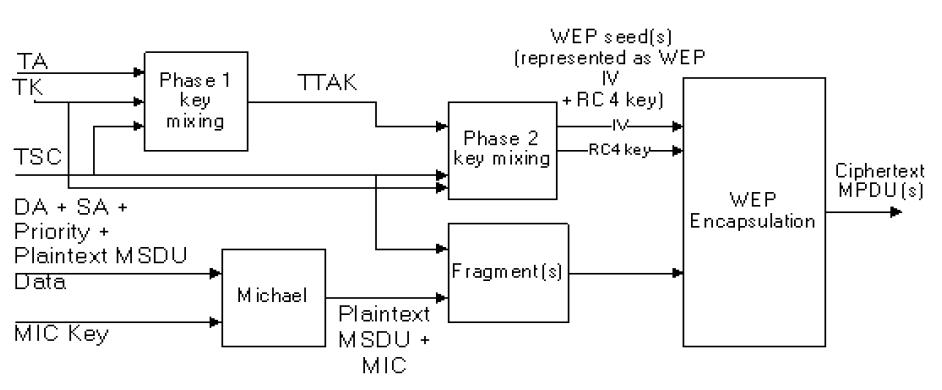
\includegraphics[scale = 0.3]{images/802_11i-encryption}
	\caption{Algoritmo TKIP.}
	\label{img:802.11i-encryption}
\end{figure}\\
Per quanto riguarda gli algoritmi di crittografia abbiamo detto che vengono utilizzati principalmente il TKIP (Figura \ref{img:802.11i-encryption}) o il CCMP al posto dell'RC4 utilizzato nel WEP. Entrambi eliminano le problematiche di sicurezza riguardanti IV corti, chiavi craccabili, CRC, etc., ma introducono una maggiore complessità e quindi l'implementazione sull'hardware esistente non è stata banale.

Sostanzialmente WPA è una versione del protocollo 802.11i che anticipa lo standard ed utilizza gli algoritmi TKIP con gestione statica delle chiavi (detta anche WPA Home o WPA-PSK); gli AP o le schede client possono utilizzare TKIP con un semplice aggiornamento del firmware. WPA2 è invece la versione completa dello standard con l'utilizzo di 802.1X (WPA Enterprise). Gli AP devono implementare i client RADIUS (Remote Authentication Dial In User Service) e l'algoritmo CCMP, difficilmente realizzabili su hardware limitati. Abbiamo in sostanza 4 tipi di chiavi: WPA-PSK, WPA Enterprise, WPA2-PSK, WPA2 Enterprise.\\
Negli ultimi anni sono stati pubblicati due articoli che descrivono una variante dell'attacco chopchop per TKIP. Con WPA non è possibile ripetere due volte lo stesso IV (che prende il nome di TSC), perché ogni ricevitore tiene un contatore degli ultimi IV ricevuti; con IEEE 802.11e, che aggiunge il supporto per la QoS, esistono 8 code di ricezione diverse, ciascuna con TSC indipendente. L'attacco può quindi essere effettuato decifrando un byte per volta di un pacchetto usando le code diverse\footnote{Per ulteriori dettagli si veda \textquotedblleft Practical attacks against WEP and WPA", \url{http://dl.aircrack-ng.org/breakingwepandwpa.pdf}}. Quindi anche TKIP inizia a mostrare le prime vulnerabilità; nella pratica è possibile decifrare un pacchetto cifrato e recuperare un keystream e riutilizzarlo in una coda distinta per iniettare un pacchetto nella rete.

\textbf{802.1X} (Port-Based Network Access Control) è uno standard che definisce dei ruoli generici per l'architettura di controllo degli accessi in reti 802. In sostanza è un'architettura, implementata da protocolli, che separa il ruolo dell'\textit{authenticator} da quello dell'\textit{authentication server}: in pratica i ruoli sono svolti da due (o tre) entità logiche distinte e specializzate. Prima dell'introduzione di questo standard questi due ruoli venivano svolti dall'AP. L'802.1X è uno standard dell'802.1, ma di seguito verrà trattato nell'ambito dell'802.11.\\
Come già accennato vengono divisi i ruoli di \textit{authenticator} e AP; quest'ultimo offre semplicemente l'accesso di livello 2. In questo modo si ridisegna la topologia della rete, rendendola gestibile in modo migliore.
\begin{figure}[htbp]
	\centering
		\begin{tikzpicture}[node distance=4cm]
			\node (supplicant) [phase,label=below:Supplicant] {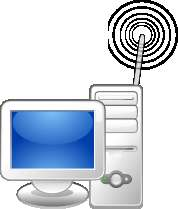
\includegraphics[scale=0.2]{images/supplicant}};	
			\node (AP) [phase, right= of supplicant,label=below:Authenticator] {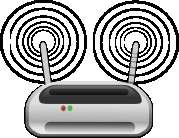
\includegraphics[scale=0.2]{images/AP}};
			\draw [undirectedarrow,draw=red] (supplicant) -- node[]{}(AP);
			\node (AS) [phase, right= of AP,label=below:Authentication Server] {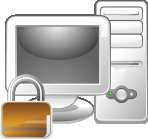
\includegraphics[scale=0.2]{images/authentication-server}};
			\draw [undirectedarrow,draw=black] (AP) -- node[]{}(AS);
		\end{tikzpicture}
	\caption{Topologia dello standard 802.1X. I collegamenti in nero sono cablati, quelli in {\textcolor{red}{rosso}} sono wireless. Il collegamento tra authenticator e authentication server è un collegamento di livello 3 che viene considerato \textit{sicuro}.}
	\label{img:802.1x-topology}
\end{figure}\\
In Figura \ref{img:802.1x-topology} è riportata la topologia di rete dello standard 802.1X. Il \textit{supplicant} si deve autenticare per entrare nella rete e deve generare il \text{keying material} per poter comunicare in modo sicuro con l'\textit{authenticator}; il termine \textquotedblleft keying material" è un'espressione generica che indica \textit{chiavi segrete di formato, lunghezza e quantità non specificate} e la loro specifica può dipendere dalla configurazione in atto oppure è definita in fase di progettazione della rete. L'\textit{authenticator} non ha un ruolo attivo nell'autenticazione: ha in pratica solo la funzione di proxy. Al fine dell'autenticazione, l'authenticator deve possedere il \textit{keying material} (viene installato dall'\textit{authentication server}) in comune con il supplicant, da cui deriverà delle chiavi per cifrare ed autenticare. L'\textit{authentication server} è sostanzialmente un database di credenziali di autenticazione e si occupa di autenticare il supplicant. Una volta stabilita l'identità del supplicant provvede a farlo entrare o meno comunicandolo all'authenticator; anche l'authentication server si deve autenticare con il supplicant: l'autenticazione è sempre bidirezionale. Si noti che lo standard 802.1X assume che il collegamento tra authenticator ed authentication server sia a livello 3 e considerato sicuro. Un altro aspetto che viene assunto dallo standard è che il canale tra supplicant ed authenticator sia sicuro, altrimenti un attaccante potrebbe usare i servizi del supplicant.\\
Consideriamo sempre la Figura \ref{img:802.1x-topology} per descrivere le quattro fasi previste dallo standard 802.1X:
\begin{enumerate}
	\item Viene effettuata un'autenticazione 802.11 (solo per compatibilità) e l'associazione tra supplicant e authenticator in modo open-system o shared key.
	\item Viene eseguita una mutua autenticazione tra supplicant ed authentication server: le due macchine verificano la reciproca identità e producono una chiave simmetrica \textit{PMK} (Pairwise Master Key). Un problema di questa fase risiede nel fatto che il collegamento tra supplicant ed authentication server è quasi in chiaro. Inoltre l'authentication server si fida dell'authenticator, perché l'authenticator gli manda un certificato, ma il collegamento tra authentication server ed authenticator deve essere sicuro, dunque l'authentication server deve sempre controllare la sicurezza del collegamento.
	\item La PMK viene spostata sull'authenticator.
	\item A partire dalla PMK, supplicant ed authenticator derivano delle chiavi che verranno utilizzate per cifrare ed autenticare tutti i pacchetti successivi, in particolare una chiave \textit{PTK} per il traffico unicast ed una chiave \textit{GTK} per il traffico multicast o broadcast. Le chiavi PTK solitamente vengono rigenerata molto spesso, al contrario della PMK, per evitare attacchi.
\end{enumerate}
Da questo momento in poi l'authentication server non partecipa più alle comunicazioni se non esplicitamente interpellato. Come già accennato, supplicant ed authenticator possono decidere, di tanto in tanto, di generare delle nuove PTK e GTK a partire dalla PMK che rimane la stessa (\textit{key refresh}); si noti che comunque l'authenticator può decidere di forzare anche una nuova autenticazione e costringere il supplicant a ripetere l'autenticazione iniziale per generare una nuova chiave PMK. Un'autenticazione completa coinvolge diversi protocolli e può essere configurata in molti modi diversi.\\
I protocolli utilizzati in 802.1X possono essere di due tipi:
\begin{itemize}
	\item \textbf{End to End (ete)}. È un protocollo che coinvolge due macchine virtualmente collegate, ma non fisicamente comunicanti (ad es. TCP/UDP); nel nostro caso è l'EAP (Extensible Authentication Protocol).
	\item \textbf{Point to Point (ptp)}. È un protocollo che coinvolge due macchine che sono direttamente connesse (ad es. DHCP); nel nostro caso è l'EAPoL (EAP over LAN), ma anche (astrattamente) il RADIUS od il DIAMETER (successore del RADIUS, utilizzato attualmente).
\end{itemize}
In particolare, nella fase 1 è utilizzato lo standard 802.11a/b/g, mentre nella fase 2 vengono utilizzati più protocolli: tra supplicant ed authentication server viene usato il protocollo EAP (ete); questo viene veicolato dentro pacchetti in formato EAPoL tra supplicant ed authenticator, e tra authenticator ed authentication server attraverso il protocollo RADIUS (ptp). Va precisato che il collegamento tra l'authentication server RADIUS ed il database LDAP deve essere sicuro, altrimenti salta tutto.\\
Nel caso in cui non si voglia utilizzare un authentication server è possibile impostare le chiavi PMK direttamente nel supplicant e nell'authenticator; si parla in questo caso di PSK (Pre-Shared Key) (WPA Home). Così facendo tutto funziona nello stesso modo, ma viene evitata la parte di autenticazione EAP proseguendo quindi con gli handshake. Le PSK possono essere configurate in una lista associandole ai MAC address delle schede di rete dei client. Una PSK è costituita da 256 bit e può essere specificata come una stringa in esadecimale (0$\times$a39f16ed6$\dots$) oppure come una password che viene trasformata in una chiave PSK di 256 bit. In Figura \ref{img:key-hierarchy} è riportata la gerarchia di generazione delle chiavi.
\begin{figure}[htbp]
	\centering
	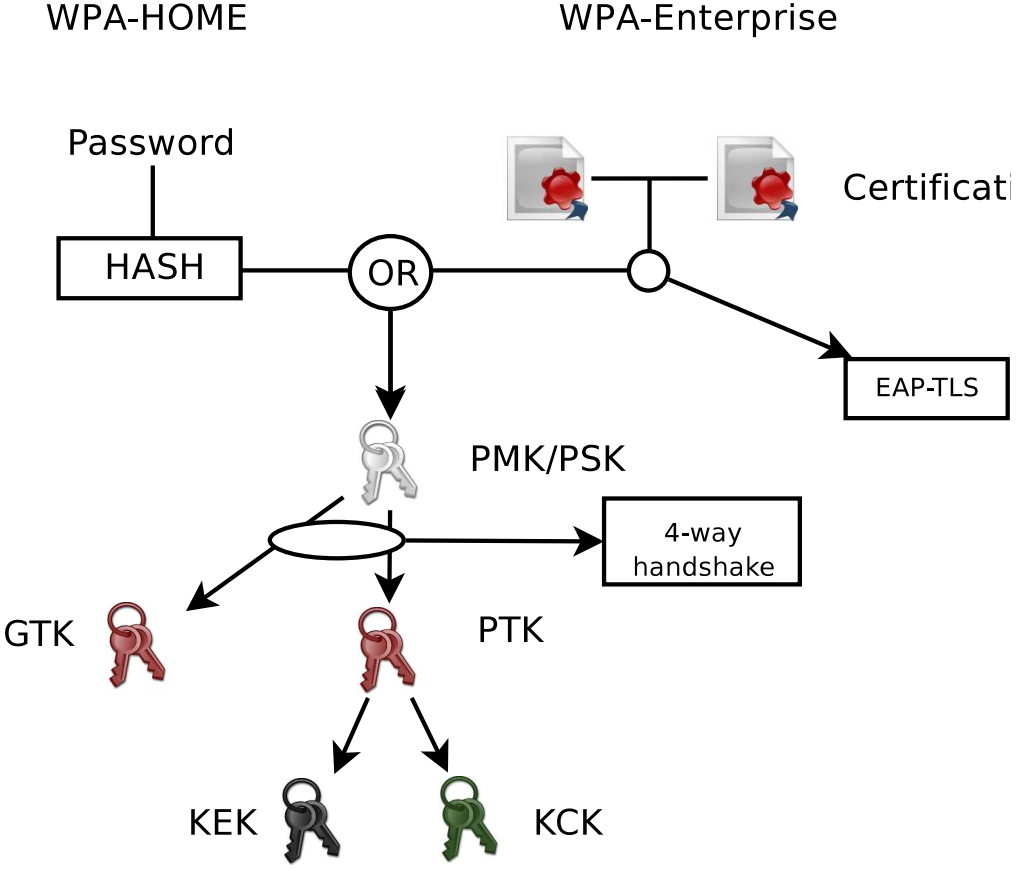
\includegraphics[scale = 0.23]{images/key-hierarchy}
	\caption{Gerarchia delle chiavi.}
	\label{img:key-hierarchy}
\end{figure}\\
Lo standard 802.1X specifica una modalità consigliata di traduzione dal segreto alla PSK:
$$\text{PSK} = \text{PBKDF2(PassPhrase, ssid, ssidLength, 4096, 256)}$$
Si noti che la PSK cambia anche se viene cambiato l'ESSID della rete. Più precisamente lo standard consiglia: \textquotedblleft \textit{A pass-phrase typically has about 2.5 bits of security per character, so the pass-phrase mapping converts an \texttt{n} octet password into a key with about 2.5\texttt{n} + 12 bits of security. Hence, it provides a relatively low level of security, with keys generated from short passwords subject to dictionary attack. Use of the key hash is recommended only where it is impractical to make use of a stronger form of user authentication. A key generated from a pass-phrase of less than about 20 characters is unlikely to deter attacks.}"
\begin{figure}[htbp]
	\centering
	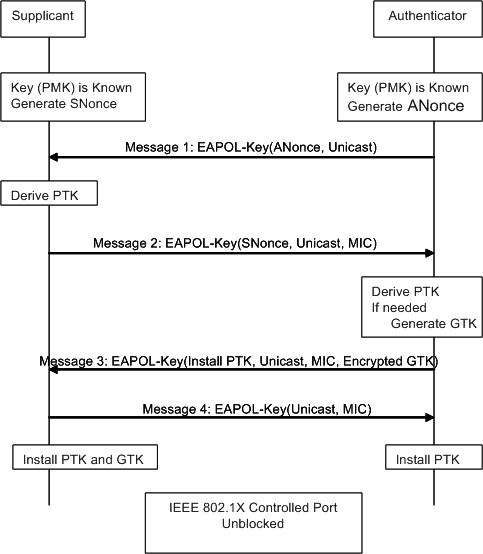
\includegraphics[scale = 0.4]{images/four-way-handshake}
	\caption{Four-way handshake.}
	\label{img:four-way-handshake}
\end{figure}\\
In Figura \ref{img:four-way-handshake} è riportato il four-way handshake; come è possibile notare, questo presenta una sorta di Diffie-Hellman per lo scambio delle chiavi. ANonce è un numero random che viene utilizzato una sola volta al fine di evitare attacchi a ripetizione.\\
Un attacco a forza bruta (brute force) sulla password può essere effettuato usando le osservazioni che seguono. La PSK viene utilizzata nel four-way handshake per generare la PTK:
$$\text{PTK} = \text{PRF}_{512}\text{(PMK, \textquotedblleft stringa", AA, SPA, ANonce, SNonce)}$$
Raccogliendo i pacchetti di un four-way handshake è possibile effettuare un attacco off-line utilizzando un dizionario di password. Per forzare un four-way handshake è possibile inviare un pacchetto di deautenticazione per forzare quindi la ripetizione di tutta la procedura. Per essere ragionevolmente sicuri di non poter essere vittima di attacchi di brute force è necessario scegliere PassPhrase con più di 20 caratteri ed utilizzare PSK in esadecimale. Entrambe le soluzioni, tuttavia, sono piuttosto scomode.

\subsubsection{Strumenti per la sicurezza}
Gli strumenti per analizzare il traffico di una rete o per individuare vulnerabilità sono molteplici. Wireshark è uno dei più conosciuti e serve per sniffare il traffico di una determinata rete; Zenmap è un'interfaccia grafica per NMAP, un software creato per effettuare port scanning, cioè mirato all'individuazione di porte aperte su un computer bersaglio o anche su range di indirizzi IP, in modo da determinare quali servizi di rete siano disponibili. Un IDS, invece, è uno strumento che serve ad effettuare una detection delle intrusioni nella rete.\\
Un IDS è sostanzialmente uno strumento che serve a difendersi dopo un attacco, al contrario di un firewall che mira a prevenire l'attacco. Un IDS può diventare un IPS (Intrusion Prevention System), cioè un rilevatore di intrusioni reattivo, che provvede ad isolare l'intruso. IPS lo potremmo dunque classificare come una versione reattiva di IDS: è uno script automatico che viene eseguito in caso di rilevazione di un attacco. Questo strumento può essere tuttavia pericoloso perché può essere attuato nei confronti di un falso positivo.\\
Il comportamento ideale di un IDS sarebbe quello che non rilevi né falsi positivi né falsi negativi; in pratica un IPS rileva dei falsi allarmi che possono tradursi nel blocco di utenti buoni, perché etichettati come malevoli. Il passaggio da IDS a IPS quindi non è facile e può risultare pericoloso. Il problema fondamentale di un IDS risiede nella configurazione stessa dell'IDS, spesso impostata per dare il minor numero possibile di allarmi all'amministratore: un numero troppo elevato indica falsi positivi e potrebbe portare l'amministratore ad ignorarli.\\
Un ulteriore problema di un IDS è la sua collocazione; teoricamente dovrebbe essere posto in ogni tratta della rete, quindi su tutti gli switch. Questo approccio è tuttavia molto costoso, dunque un'idea potrebbe essere quella di installarlo in prossimità dei firewall o nelle vicinanze dei NAS (Network Access Server), un client RADIUS che permette l'accesso alla rete. Realizzare un IDS è anche molto costoso, poiché deve scaricare il traffico ed analizzarlo in una finestra di tempo abbastanza lunga; questo si traduce in una buona capacità computazionale ed una memoria sufficientemente grande. I tre IDS prevalentemente utilizzati sono: \textit{Snort}, \textit{Suricata} e \textit{Bro}.\\
Snort e Suricata sono multithread, sono classificati come old-style e le loro regole sono compatibili: ognuno può utilizzare le regole dell'altro e viceversa. Le regole di tutti gli IDS generalmente sono stringhe rappresentanti pattern molto complicati. Suricata e Snort tentano di avere le massime performance possibili dal punto di vista dell'estrazione e dell'analisi del traffico, Bro, invece, mira ad effettuare un'analisi condivisa con altri engine. In una rete con velocità superiore al Gbps gli IDS realizzati con Suricata e Snort rappresentano un collo di bottiglia, che Bro invece cerca di superare. Un punto negativo di Bro è la non retrocompatibilità con Snort e Suricata.\\
Cosa cambia tra attacchi IPv4 e IPv6? La risposta dipende dal livello considerato; a livello applicazione cambia qualcosa ed un esempio è Snort. La differenza risiede nella compatibilità con IPv6 che non è sempre garantita, né per i firewall né per gli IDS.\\
Esiste, inoltre, un'altra categoria di IDS che si basa sul comportamento (behaviour) dell'utente anziché su alcuni pattern applicati al traffico. Grazie all'analisi del comportamento dell'utente è possibile rilevare quindi eventuali attacchi utilizzando gli IDS. Il problema principale di questo tipo di IDS risiede nella definizione delle regole: è difficile definire il comportamento degli utenti in modo preciso.